\begin{figure}
\centering

\ifpdf
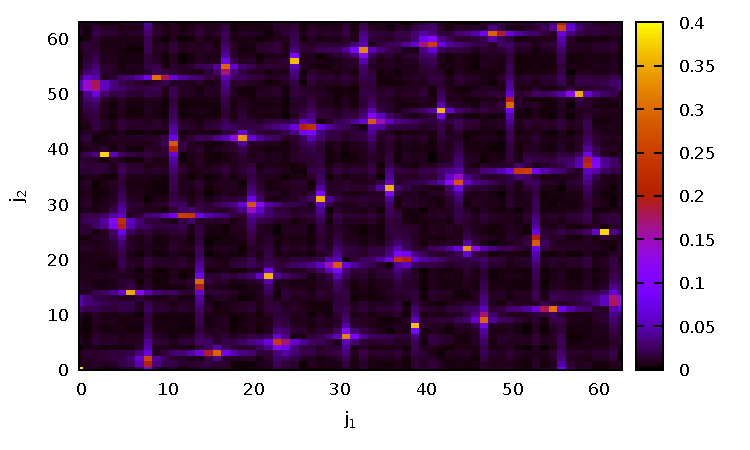
\includegraphics[angle=0]
{elliptic/picellipticdiscretlog2.pdf}
\else
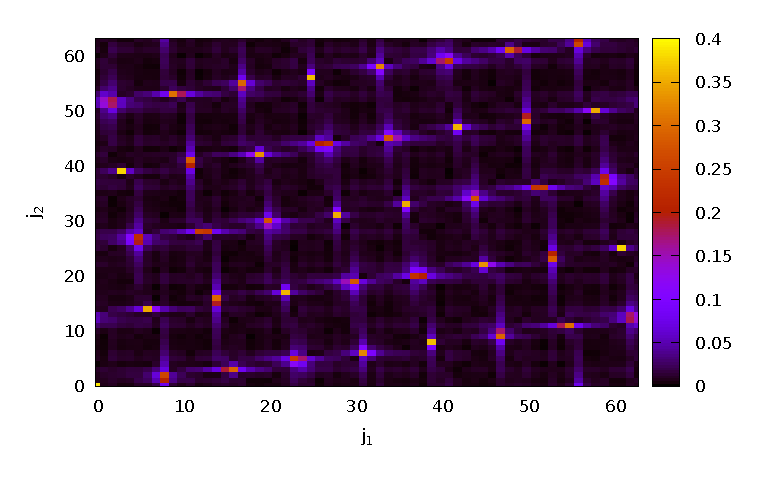
\includegraphics[angle=0]
{elliptic/picellipticdiscretlog2.eps}
\fi

\caption{Fourier transform of the samples of the function 
$f'(x_1, x_2)$
Number of samples $M=64$. The three lower left maxima have coordinates $\approx (8,2), (15,3), (24,5)$, giving the following estimates for $x$: $x \approx 4, 5, 4.8$,
which is close to the actual value $x = 5$
} 
\label{fig:quantcomp:dle2}
\end{figure}
